\documentclass{siamart1116}
\usepackage{amsmath, amssymb}
%\usepackage{amsmath,amssymb,amsfonts,graphicx,amsthm,dsfont}
%\usepackage{listings}
%\usepackage{courier}
\usepackage{enumerate}
%\usepackage{color}
%\usepackage[usenames,dvipsnames]{xcolor}
%\usepackage{hyperref,tikz,mdframed}
%\hypersetup{colorlinks=true,urlcolor=MidnightBlue,citecolor=PineGreen,linkcolor=BrickRed}

% \lstset{
% 	basicstyle=\small\ttfamily,
% 	keywordstyle=\color{blue},
% 	language=python,
% 	xleftmargin=16pt,
% }
\usepackage{algorithmicx}
\usepackage{algpseudocode}% http://ctan.org/pkg/algorithmicx
\usepackage{multicol}

\textwidth=5.8in
\textheight=9in
\topmargin=-0.5in
\headheight=0in
\headsep=.5in
\hoffset  -.4in
\pagestyle{empty}

\newcommand{\Fp}{\mathbb{F}_p}
\newcommand{\Q}{\mathbb{Q}}
\newcommand{\Z}{\mathbb{Z}}
\newcommand{\kron}[2]{\left(\frac{#1}{#2}\right)}
\newcommand{\Aut}{\mathrm{Aut}}
\newcommand{\End}{\mathrm{End}}
\newcommand{\SO}{\mathrm{SO}}
\newcommand{\SU}{\mathrm{SU}}
\newcommand{\tr}{\operatorname{tr}}
\newcommand{\dee}{\mathrm{d}}
\newcommand{\deee}{\textbf{\text{\emph{d}}}}

\newcommand{\md}[1]{\textcolor{cyan}{#1}}

\newcommand{\TheAuthors}{V. Chen}

%\newtheorem{theorem}{Theorem}
%\newtheorem{definition}{Definition}

\graphicspath{ {graphics/} }

\title{Comparing hierarchical methods}
\author{\TheAuthors}
\date{}
\begin{document}
\maketitle
\setlength{\unitlength}{1in}
\setlength{\parindent}{0in}
\section{Algorithm for hierarchical towards $\tau, \alpha, M$}
\begin{equation}
\label{eqn:noncentered_T}
T(\xi,\tau,\alpha, M) = \sum_{i=0}^M \frac{1}{(\lambda_i+\tau^2)^{\alpha/2}}\xi_iq_i = u
\end{equation}


\begin{equation}
\label{eqn:noncentered_post}
g(\xi,\tau,\alpha, M) \propto \exp\left( -\Phi(T(\xi,\tau,\alpha,M))-\frac{1}{2}\langle \xi,\xi \rangle + \log(\pi_0(\tau,\alpha,M)) \right)
\end{equation}


\begin{algorithm}

\caption{Non-centered parameterization, hierarchical with $\tau, \alpha, M$}
\label{alg:hier_t_a_M}
\begin{algorithmic}
\State Choose $\xi^{(0)} \in \mathbb{R}^N, \tau^{(0)}, \alpha^{(0)}, M^{(0)} > 0, \beta \in (0, 1]$ and $\epsilon_1, \epsilon_2 > 0$.
\For{$k=0$ to $S$}
\State Propose $\hat\xi^{(k)} = (1-\beta^2)^{\frac{1}{2}}\xi^{(k)} + \beta \zeta^{(k)}$, $\zeta^{(k)} \sim \mathsf{N}(0, I)$
\State Make transition $\xi^{(k)} \to \hat\xi^{(k)}$ with probability
\[ A(\xi^{(k)} \to \hat\xi^{(k)}) = \min\left\{1, \exp\left(\Phi(T(\xi^{(k)},\tau^{(k)},\alpha^{(k)}, M^{(k)})) - \Phi(T(\hat\xi^{(k)},\tau^{(k)},\alpha^{(k)}, M^{(k)}))\right) \right\}\] \Comment{$T$ defined in \cref{eqn:noncentered_T}}

\State Propose $\hat\tau^{(k)} = \tau^{(k)} + \epsilon_1 \rho^{(k)}, \rho^{(k)} \sim \mathsf{N}(0,1)$
\State Make transition $\tau^{(k)} \to \hat\tau^{(k)}$ with probability
\[ A(\tau^{(k)} \to \hat\tau^{(k)}) 
= \min\left\{1, \frac{g(\xi^{(k+1)},\hat\tau^{(k)},\alpha^{(k)},M^{(k)})}{g(\xi^{(k+1)},\tau^{(k)},\alpha^{(k)},M^{(k)})} \right\}\] \Comment{$g$ defined in \cref{eqn:noncentered_post}}

\State Propose $\hat\alpha^{(k)} = \alpha^{(k)} + \epsilon_2 \sigma^{(k)}, \sigma^{(k)} \sim \mathsf{N}(0,1)$
\State Make transition $\alpha^{(k)} \to \hat\alpha^{(k)}$ with probability
\[ A(\alpha^{(k)} \to \hat\alpha^{(k)}) 
= \min\left\{1, \frac{g(\xi^{(k+1)},\tau^{(k+1)},\hat \alpha^{(k)},M^{(k)})}{g(\xi^{(k+1)},\tau^{(k+1)},\alpha^{(k)},M^{(k)})} \right\}\]
\State Propose $\hat M^{(k)} = M^{(k)} + Q$, with jump $Q$ distributed as $\mathbb{P}(Q=k) \propto \frac{1}{1+|k|}$, $|Q|$ bounded.
\State Make transition $M^{(k)} \to \hat M^{(k)}$ with probability
\[ A(M^{(k)} \to \hat M^{(k)}) = 
\min\left\{1, \frac{g(\xi^{(k+1)},\tau^{(k+1)},\alpha^{(k+1)},\hat M^{(k)})}{g(\xi^{(k+1)},\tau^{(k+1)},\alpha^{(k+1)},M^{(k)})} \right\}
\]
\EndFor
\State \Return $\{ T(\xi^{(k)},\tau^{(k)},\alpha^{(k)}, M^{(k)}), \tau^{(k)}, \alpha^{k} \}$
\end{algorithmic}
\end{algorithm}

\section{$M$ and $\sigma$ relation}
We tested our algorithm on the two moons dataset with varying $\sigma$, fixing $3\%$ labeled nodes. We also fixed $\tau=1,\alpha=35$ by setting $\epsilon_1=\epsilon_2=0$, so the algorithm is only learning $\xi$ and $M$. We initialized $M^{(0)} = 30$. We can see that for small $\sigma = 0.02$, $M$ is very small as only the first few eigenvectors are necessary (see \cref{fig:learnM_sigma_0.02}). However, when we choose a larger $\sigma = 0.2$, $M$ needs to be larger (see \cref{fig:learnM_sigma_0.20}). For $\sigma = 0.02$, the classification accuracy was 100\%. For $\sigma = 0.2$, the classification accuracy was 90.21\%.

\begin{figure}[!htb]
\caption{\label{fig:learnM_sigma_0.02} $\sigma=0.02$, trace of $M$}
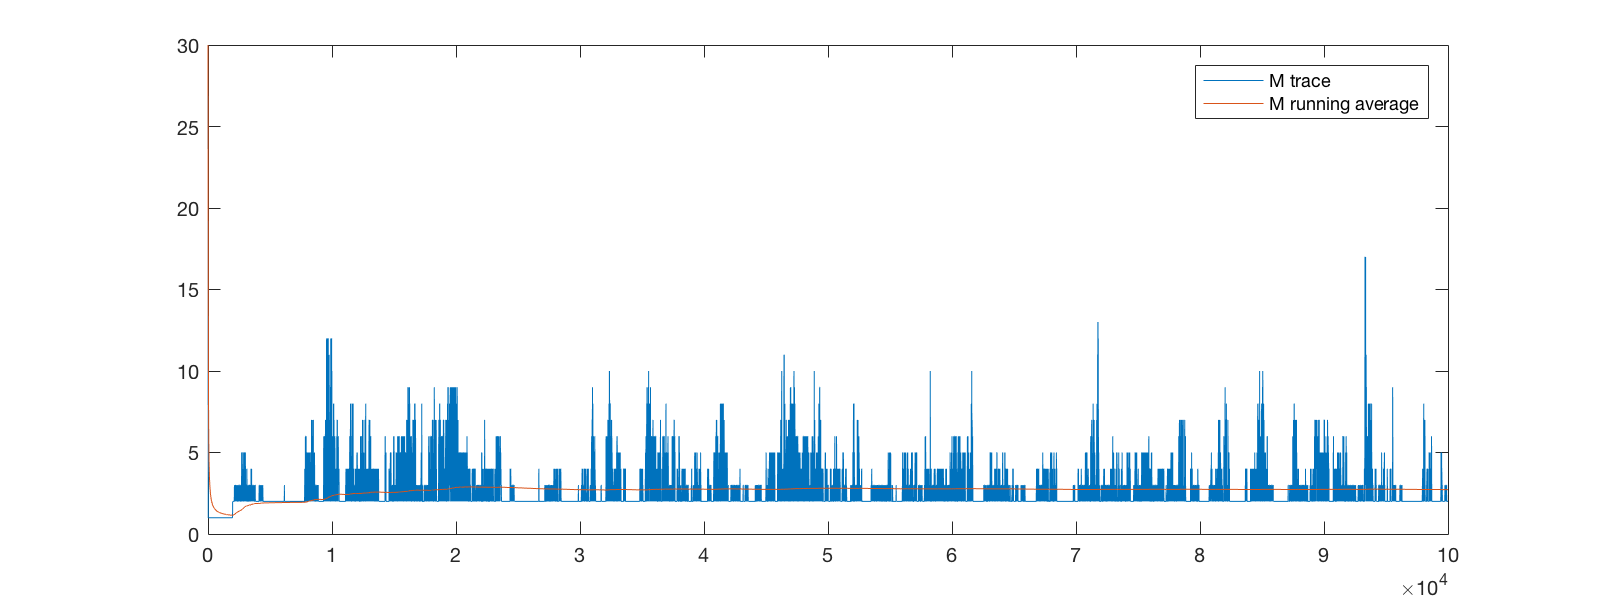
\includegraphics[width=\linewidth]{old/sigma_0_02/M_trace.png}
\end{figure}
\begin{figure}[!htb]
\caption{\label{fig:learnM_sigma_0.20} $\sigma=0.2$, trace of $M$}
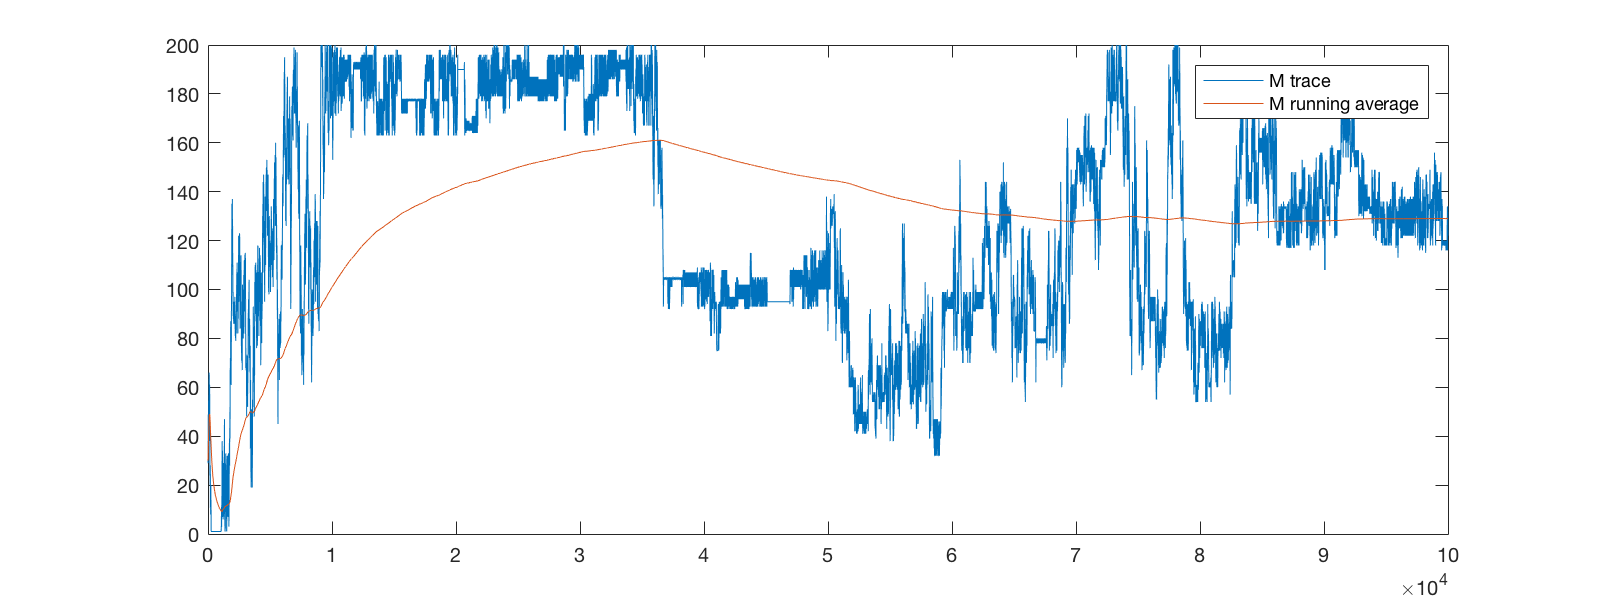
\includegraphics[width=\linewidth]{old/sigma_0_20/M_trace.png}
\end{figure}

\section{Nonhierarchical vs. Hierarchical}
We will compare pCN with fixed $\tau$ and $\alpha$ against \cref{alg:hier_t_a_M} with the same fixed $\tau$ and $\alpha$, but learning $M$.
\subsection{Voting records}
The nonhierarchical algorithm for learning $\tau$ and $\alpha$ gave expected values of $\tau$ and $\alpha$ as $\tau \approx 2$ and $\alpha \approx 35$, so I chose those parameters for the pCN and for \cref{alg:hier_t_a_M}. For the pCN, all $435$ eigenvectors were used. I narrowed the range of $M$ allowed in \cref{alg:hier_t_a_M} to 1 to 70. 5 labeled nodes were selected, consistent across the two methods. The results are not very concrete yet. Tentatively, it seems that being hierarchical does have some benefits, but more experiments are needed. In this particular realization (seeded with $\text{rng}(5)$), the hierarchical algorithm achieves $90.70\%$ while the nonhierarchical algorithm achieves $87.67\%$ classification accuracy. \cref{fig:voting_nonhier_u_avg}, \cref{fig:voting_nonhier_u_accept}, \cref{fig:voting_nonhier_senator_traces}, \cref{fig:voting_hier_M_trace}, \cref{fig:voting_hier_M_accept}, \cref{fig:voting_hier_u_avg}, \cref{fig:voting_hier_xi_accept} show the results of this experiment. Notice in \cref{fig:voting_hier_M_trace} that there seems to be an important eigenvector for classification indexed around 30, as $M$ seldom drops below $30$. Looking at the eigenvectors around index 30, I plotted the 34th eigenvector in \cref{fig:voting_hier_eigenvector}. From a purely visual perspective, it does appear that this eigenvector corresponds decently to the final classification in \cref{fig:voting_hier_u_avg} by looking at where some of the ``spikes'' are.

\begin{figure}[!htb]
\begin{minipage}{0.48\textwidth}
    \centering
    \caption{\label{fig:voting_nonhier_u_avg} Average of $S(u)$}
    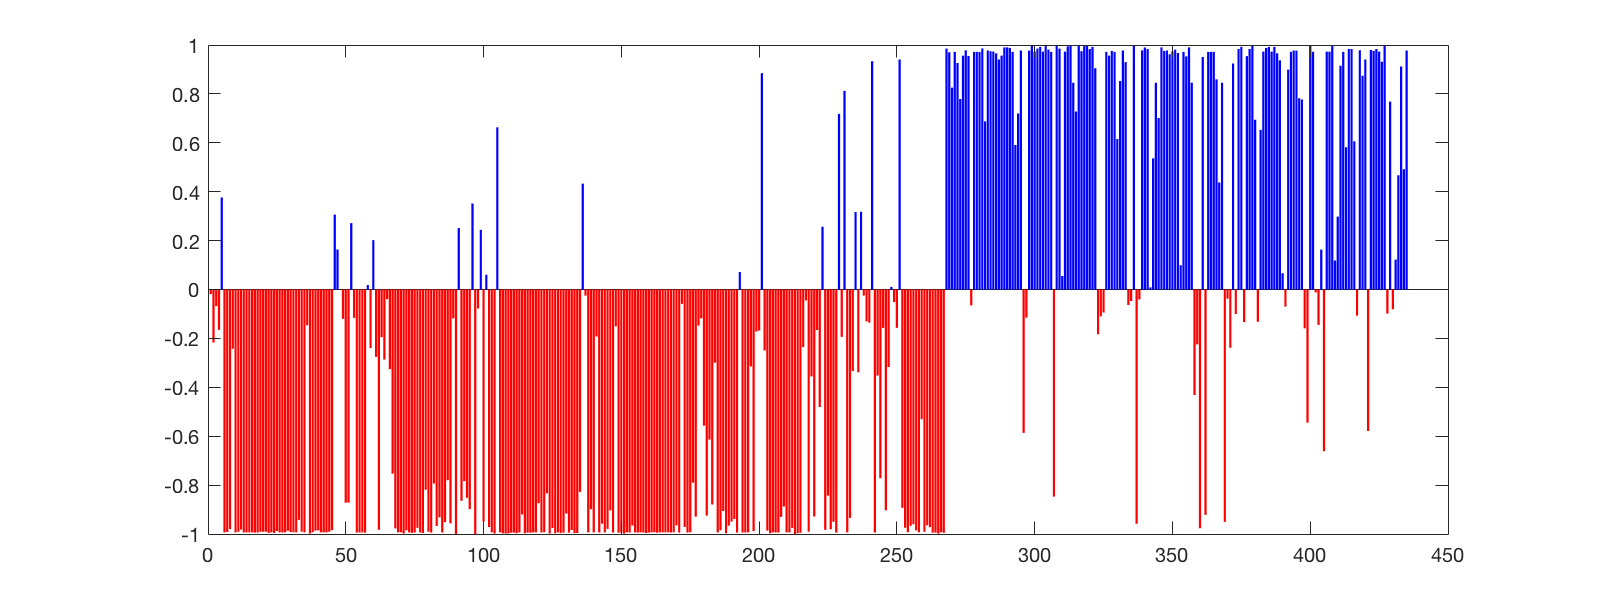
\includegraphics[width=\linewidth]{voting/nonhier/u_avg.png}
\end{minipage} \hfill
\begin{minipage}{0.48\textwidth}
    \centering
    \caption{\label{fig:voting_nonhier_u_accept} $u$ acceptance probability}
    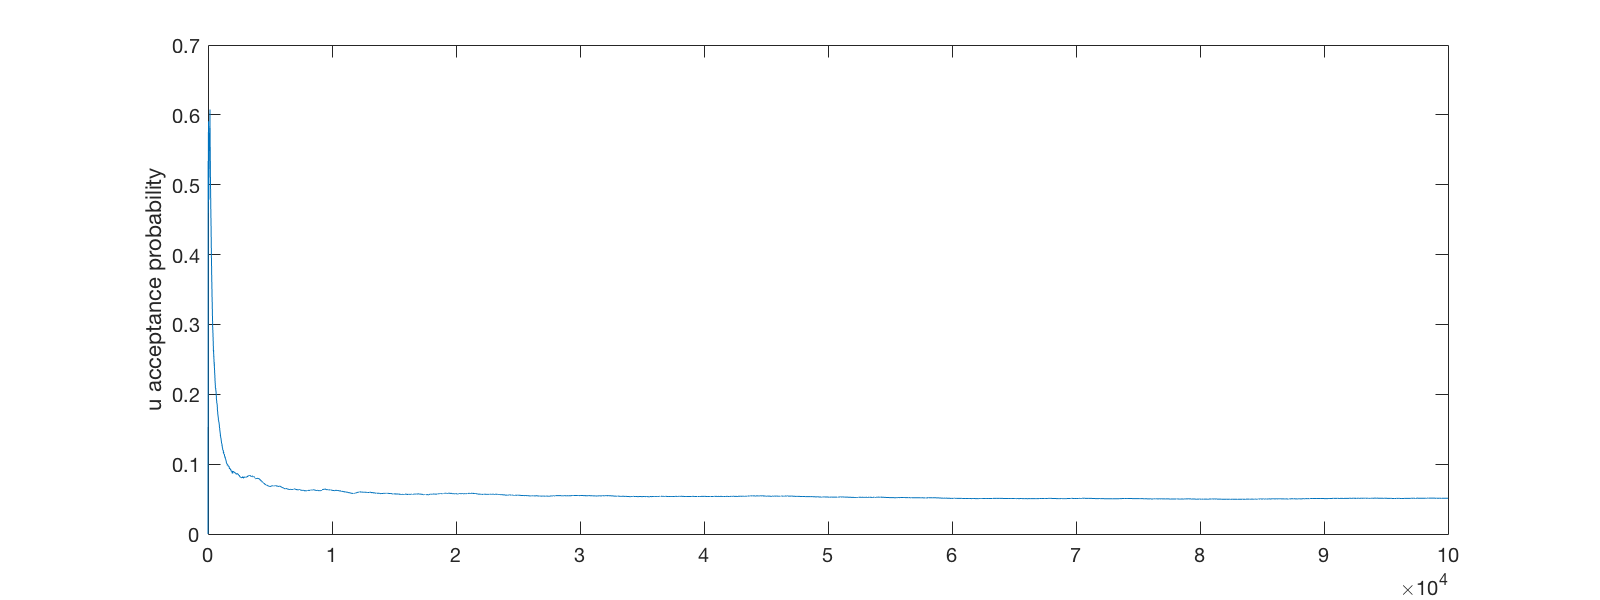
\includegraphics[width=\linewidth]{voting/nonhier/u_accept.png}
\end{minipage}
\end{figure}

\begin{figure}[!htb]
\caption{\label{fig:voting_nonhier_senator_traces} Running average of $S(u(i))$ for select $i$}
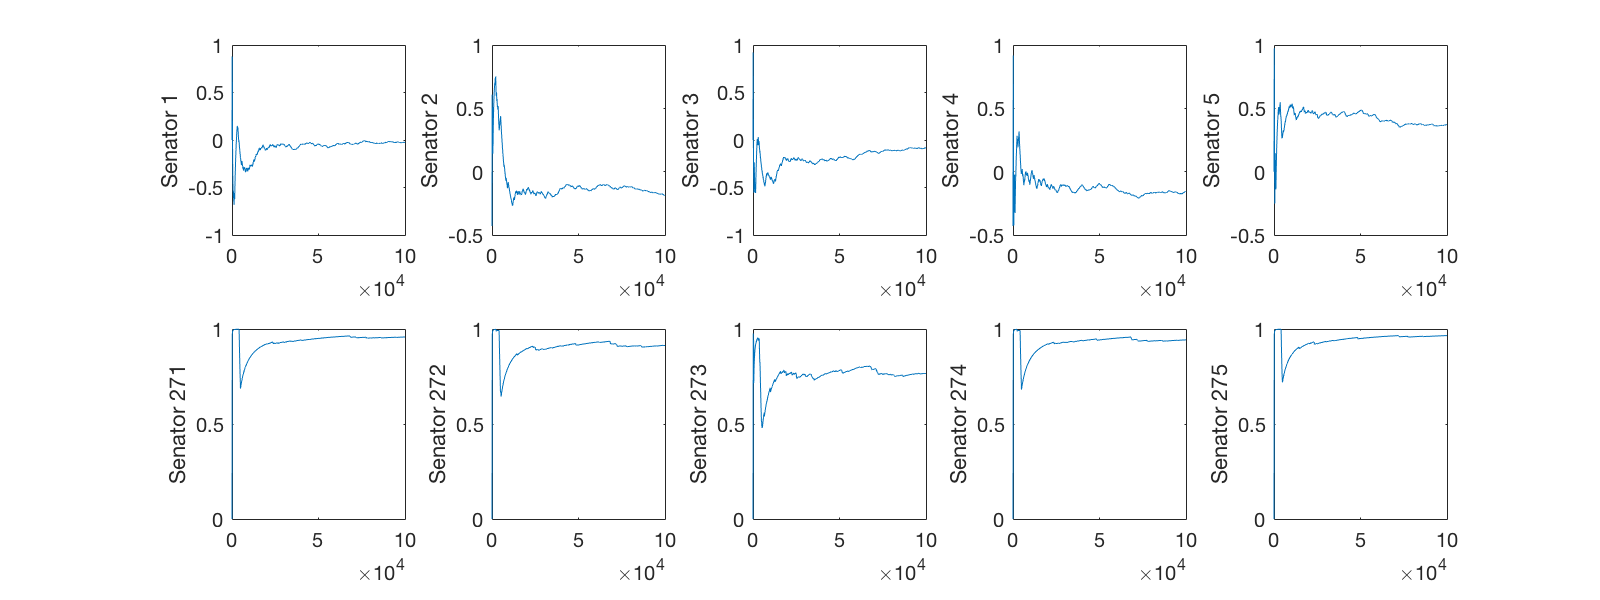
\includegraphics[width=\linewidth]{voting/nonhier/senator_traces.png}
\end{figure}

\begin{figure}[!htb]
\begin{minipage}{0.48\textwidth}
    \centering
    \caption{\label{fig:voting_hier_M_trace} Trace of $M$}
    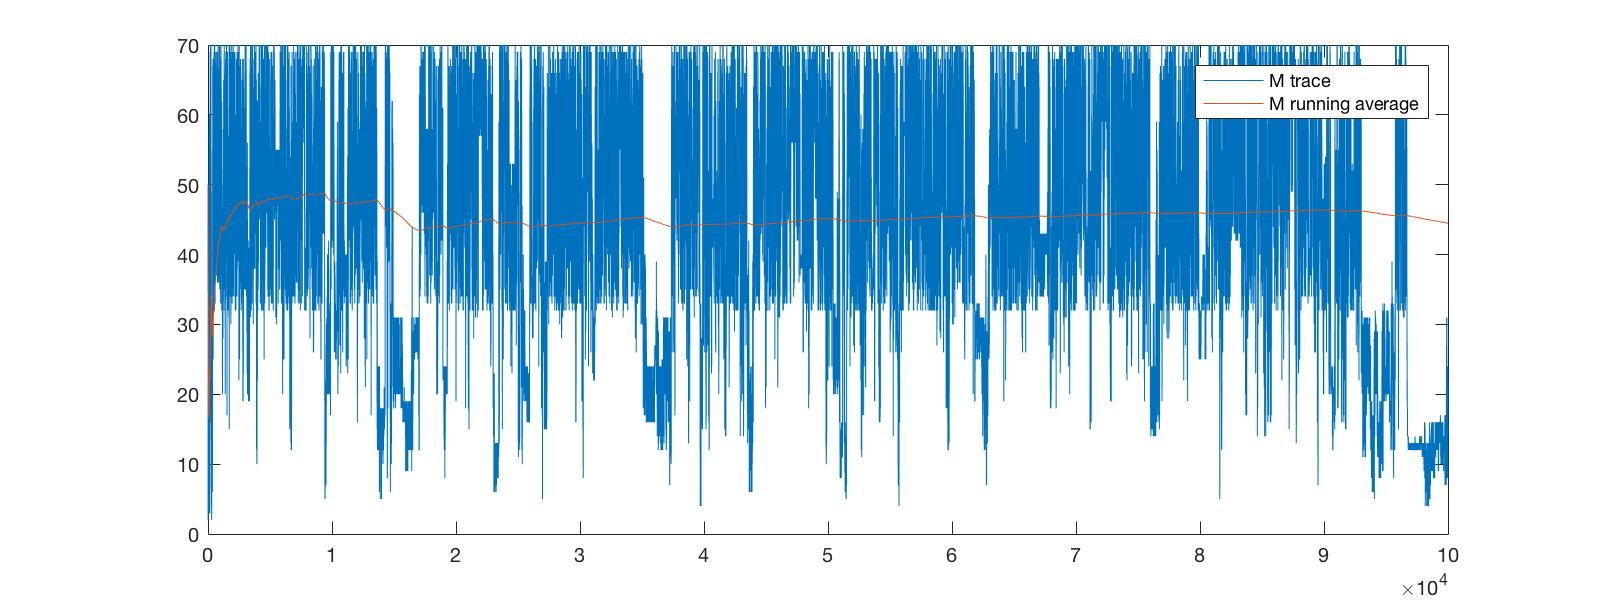
\includegraphics[width=\linewidth]{voting/hier/M_trace.png}
\end{minipage} \hfill
\begin{minipage}{0.48\textwidth}
    \centering
    \caption{\label{fig:voting_hier_M_accept} $M$ acceptance probability}
    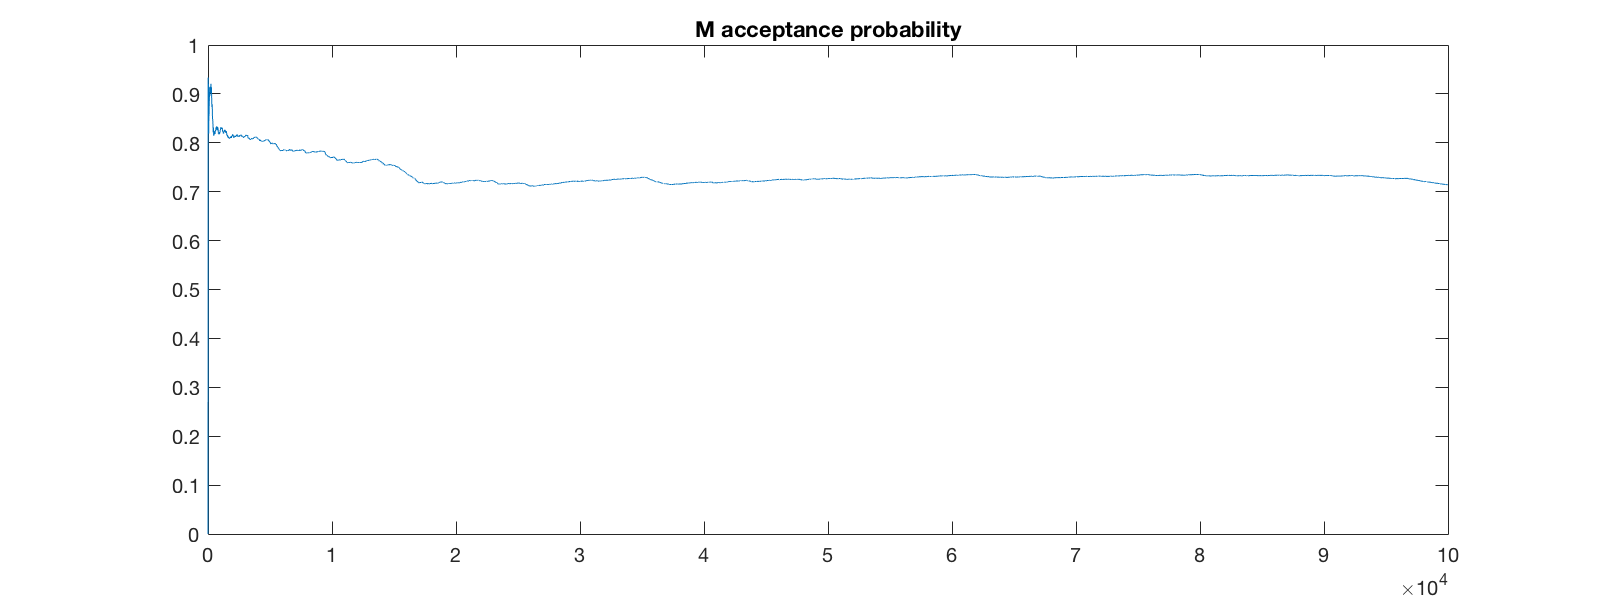
\includegraphics[width=\linewidth]{voting/hier/M_accept.png}
\end{minipage}
\end{figure}

\begin{figure}[!htb]
\begin{minipage}{0.48\textwidth}
    \centering
    \caption{\label{fig:voting_hier_u_avg} Average of $S(u)$}
    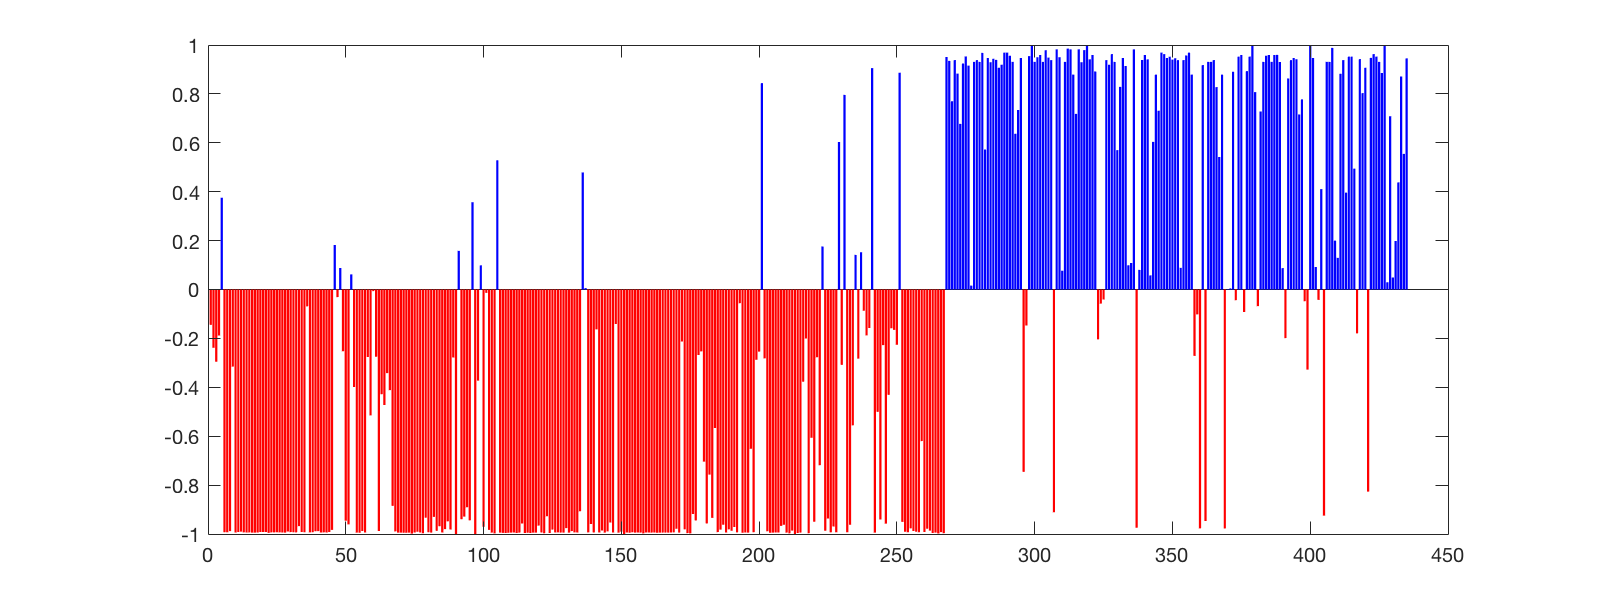
\includegraphics[width=\linewidth]{voting/hier/u_avg.png}
\end{minipage} \hfill
\begin{minipage}{0.48\textwidth}
    \centering
    \caption{\label{fig:voting_hier_xi_accept} $\xi$ acceptance probability}
    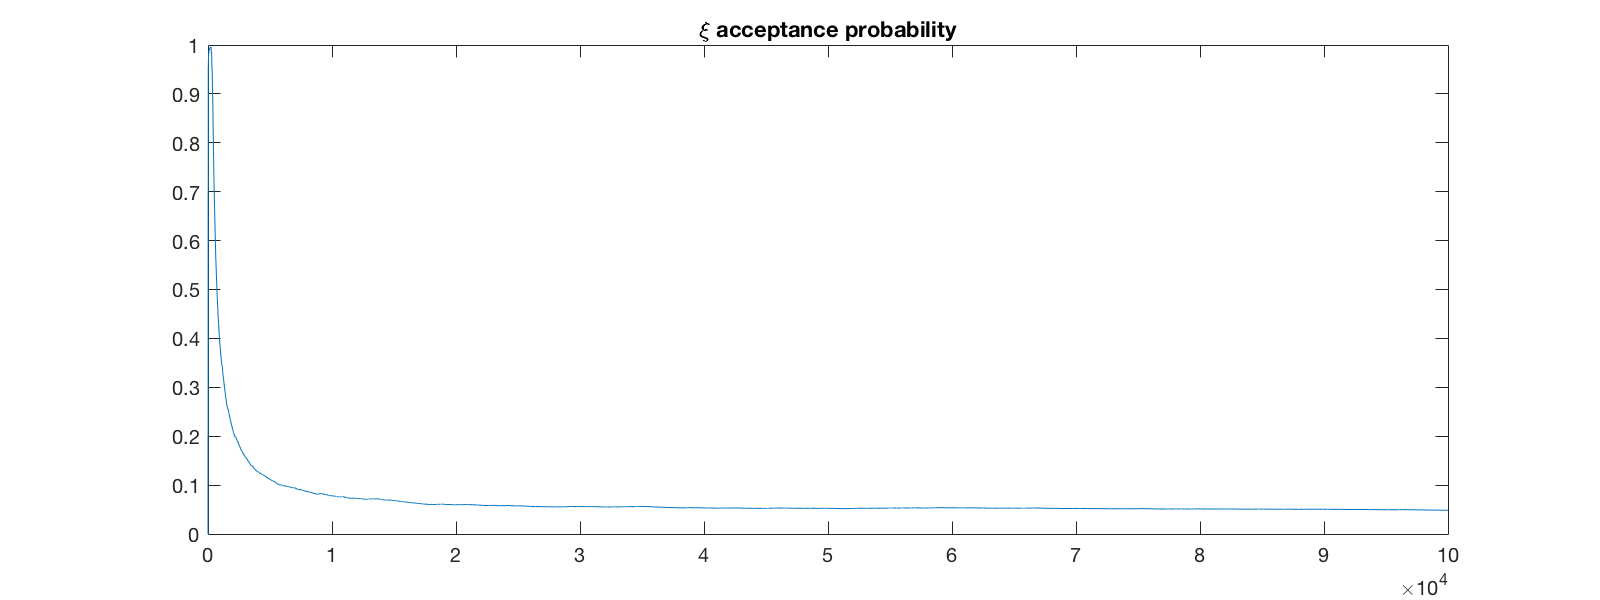
\includegraphics[width=\linewidth]{voting/hier/xi_accept.png}
\end{minipage}
\end{figure}

\begin{figure}[!htb]
\caption{\label{fig:voting_hier_eigenvector} 34th eigenvector of unnormalized fixed length-scale $L$}
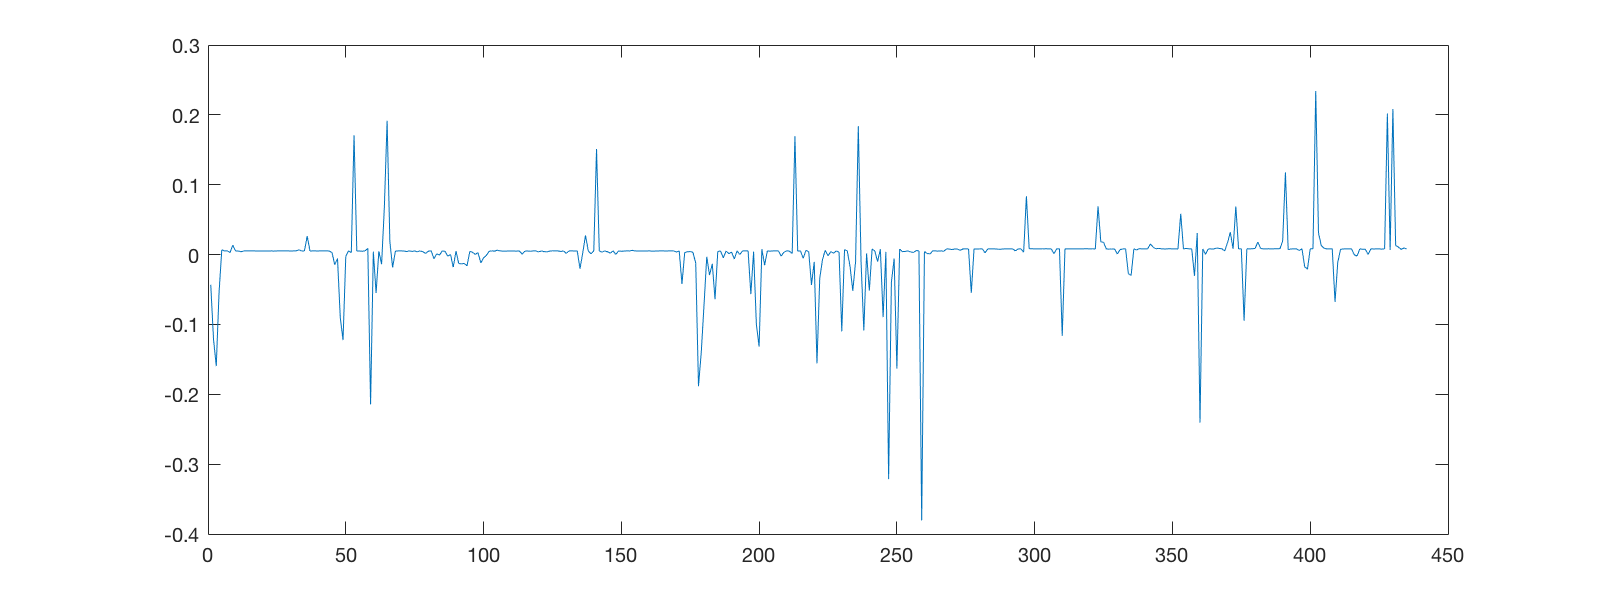
\includegraphics[width=\linewidth]{voting/hier/34_eigvec.png}
\end{figure}

\subsection{Two moons}
I tried a similar set of experiments on the two moons data. I fixed $\tau = 2, \alpha = 35$, again following the expected values of these hyperparameters from the noncentered algorithm that learns $\tau,\alpha$. I set the pCN to use the first $100$ eigenvectors, and I set the range for $M$ in \cref{alg:hier_t_a_M} to be $[1, 70]$. The two moons data was generated with $N=2000, d=100, \sigma = 0.2$ and $1\%$ fidelity. The nodes selected for fidelity are random but consistent between the different methods, as is the data itself. The colored diamonds in the scatter plots are the labeled nodes. I ran this test with two different seeds. With seed $\text{rng}(3)$, the two algorithms perform similarly well, as shown in the final clustering in \cref{fig:moons_nonhier1_scatter} and \cref{fig:moons_hier1_scatter}. In \cref{fig:moons_hier1_M_trace}, $M$ seems to have moved from its uniform prior distribution, preferring a mean of around $15$. With $\text{rng}(4)$, the hierarchical algorithm is more accurate than the nonhierarchical one, as seen in the clustering shown in \cref{fig:moons_nonhier2_scatter} and \cref{fig:moons_hier2_scatter}. The trace of $M$ in \cref{fig:moons_hier2_M_trace} seems to show convergence after 50000 iterations, but perhaps it is difficult to say because from around 30000 to 40000 it also looked like it converged. The results again suggest that there is some value to being hierarchical with $M$ even with good choices of $\tau$ and $\alpha$, but more experiments are needed. 

% rng(3)

\begin{figure}[!htb]
\begin{minipage}{0.48\textwidth}
    \centering
    \caption{\label{fig:moons_nonhier1_scatter} Nonhierarchical, seed $\text{rng}(3)$. Final classification projected into first two dimensions.}
    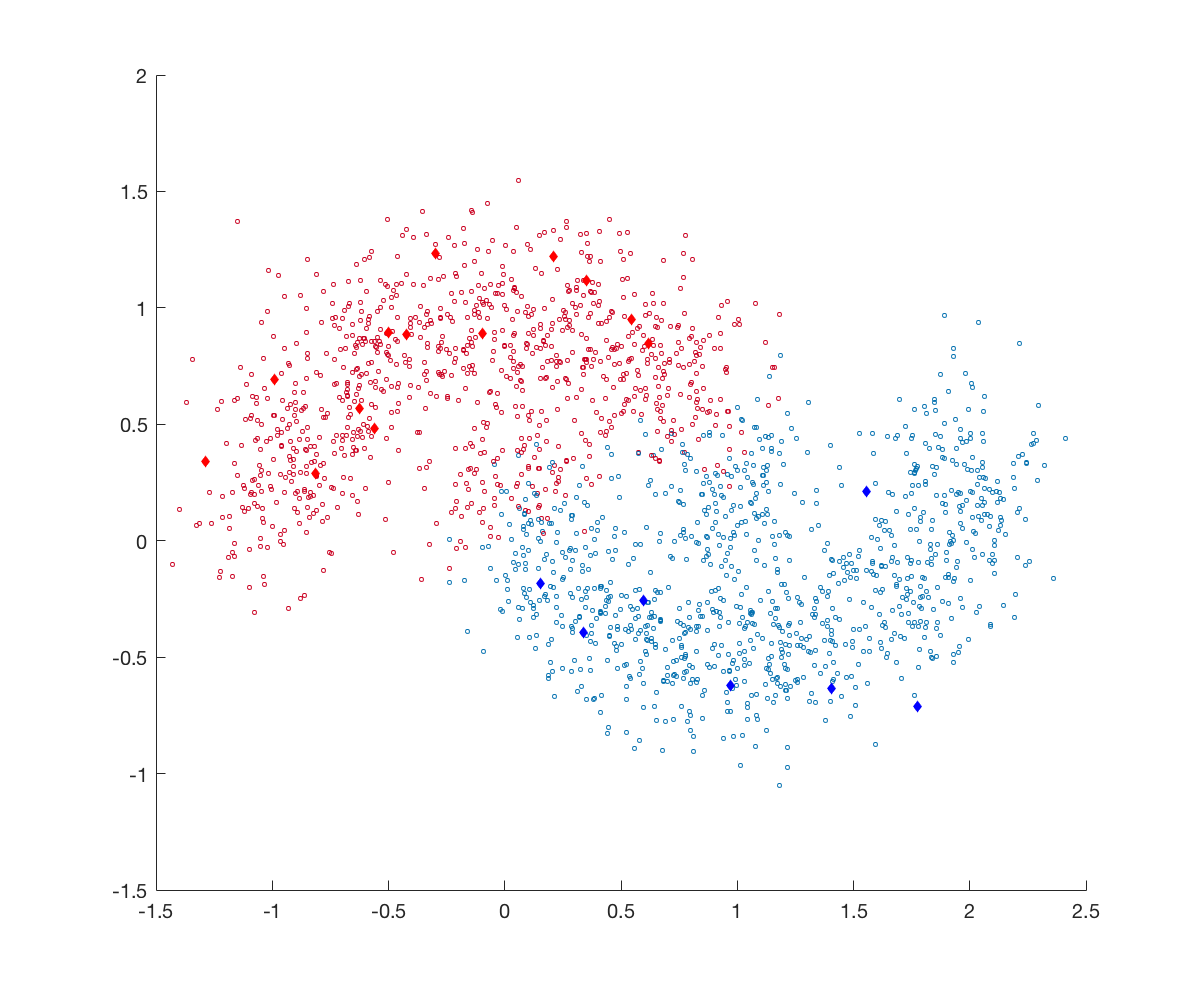
\includegraphics[width=\linewidth]{moons/nonhier1/scatter.png}
\end{minipage} \hfill
\begin{minipage}{0.48\textwidth}
    \centering
    \caption{\label{fig:moons_nonhier1_u_accept} Nonhierarchical, seed $\text{rng}(3)$. $u$ acceptance probability.}
    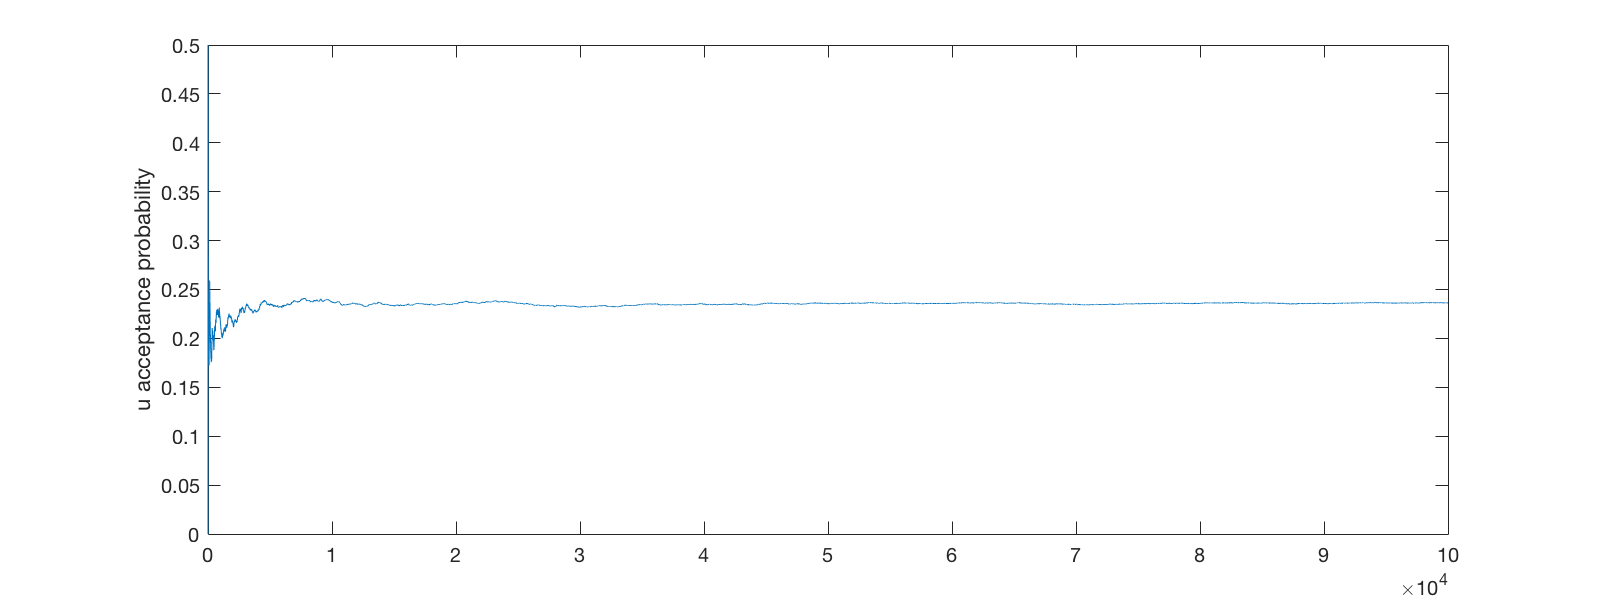
\includegraphics[width=\linewidth]{moons/nonhier1/u_accept.png}
\end{minipage}
\end{figure}

\begin{figure}[!htb]
\begin{minipage}{0.48\textwidth}
    \centering
    \caption{\label{fig:moons_hier1_scatter} Hierarchical, seed $\text{rng}(3)$. Final classification projected into first two dimensions.}
    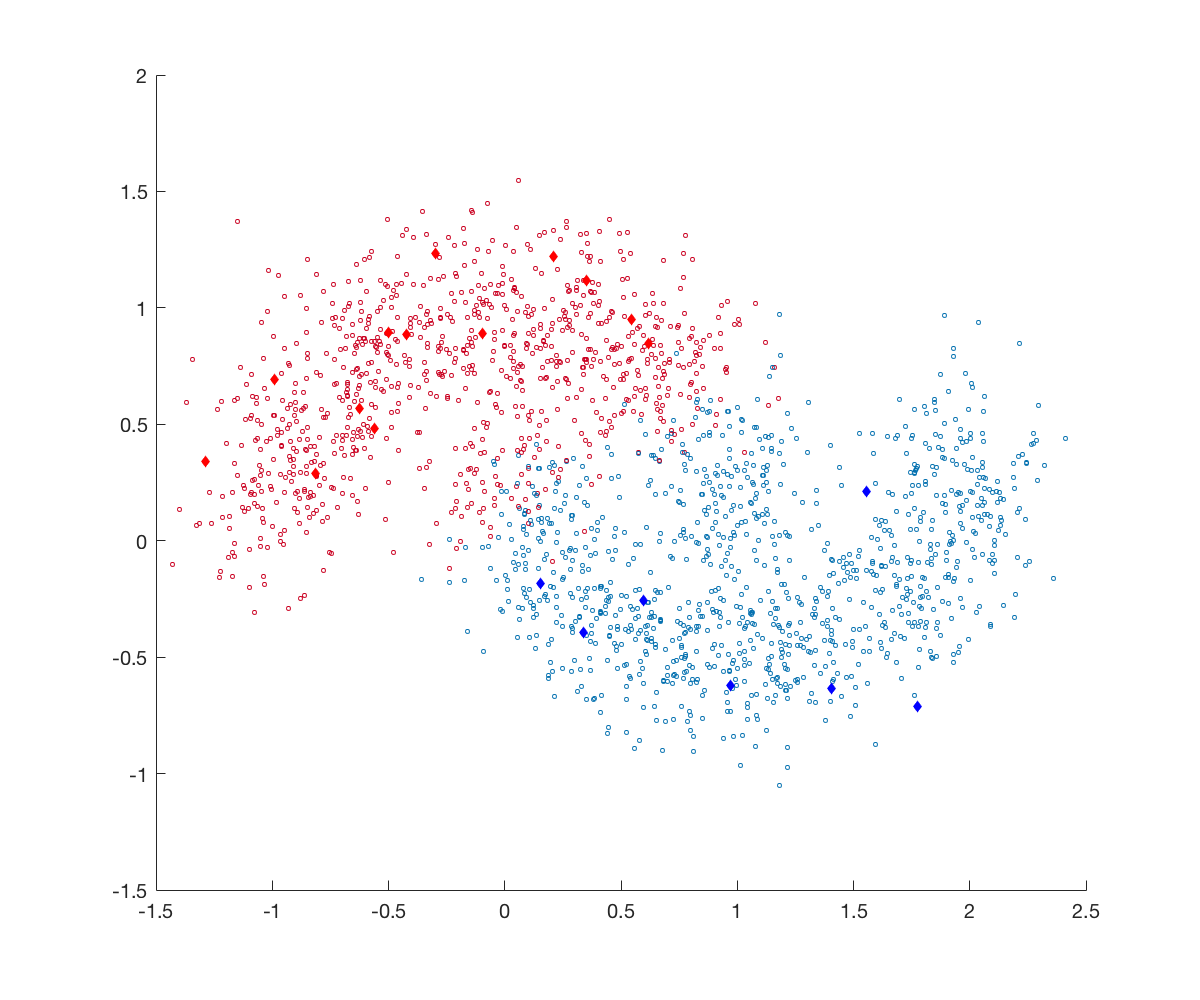
\includegraphics[width=\linewidth]{moons/hier1/scatter.png}
\end{minipage} \hfill
\begin{minipage}{0.48\textwidth}
    \centering
    \caption{\label{fig:moons_hier1_u_accept} Hierarchical, seed $\text{rng}(3)$. $\xi$ acceptance probability.}
    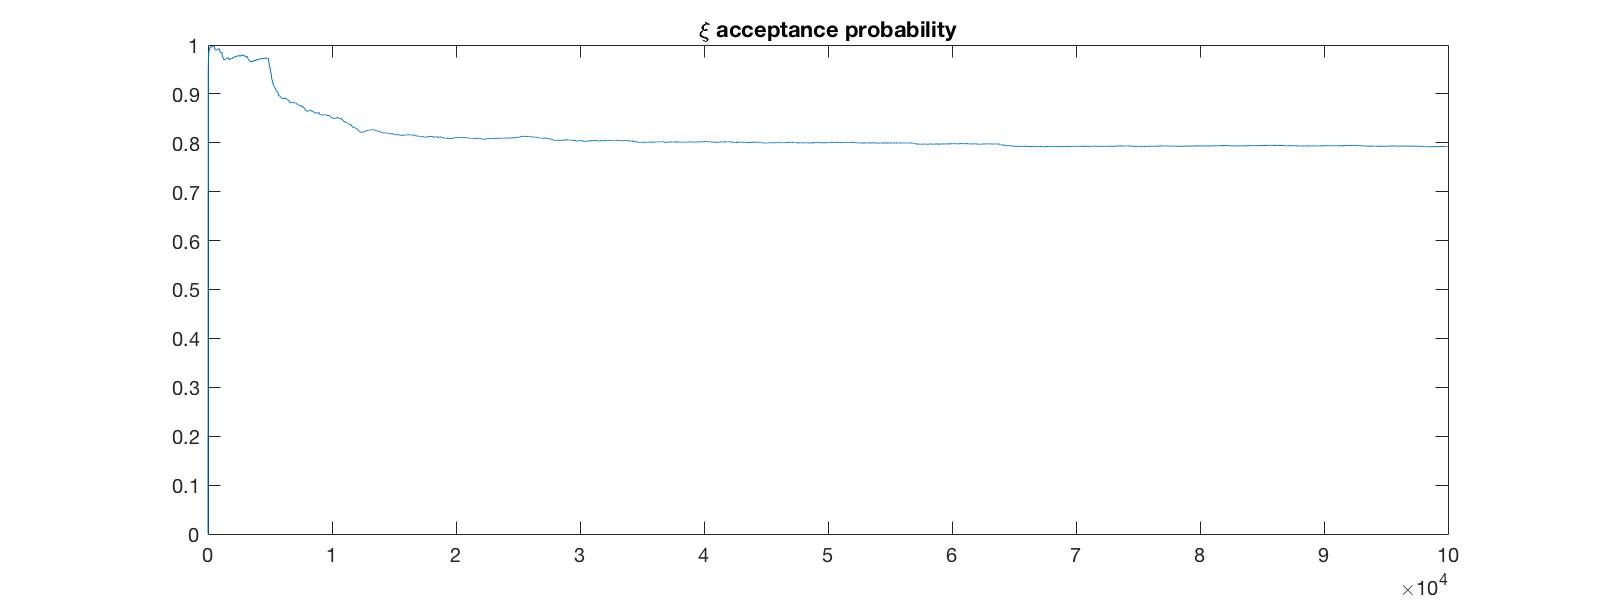
\includegraphics[width=\linewidth]{moons/hier1/xi_accept.png}
\end{minipage}
\end{figure}

\begin{figure}[!htb]
\begin{minipage}{0.48\textwidth}
    \centering
    \caption{\label{fig:moons_hier1_M_trace} Hierarchical, seed $\text{rng}(3)$. $M$ trace.}
    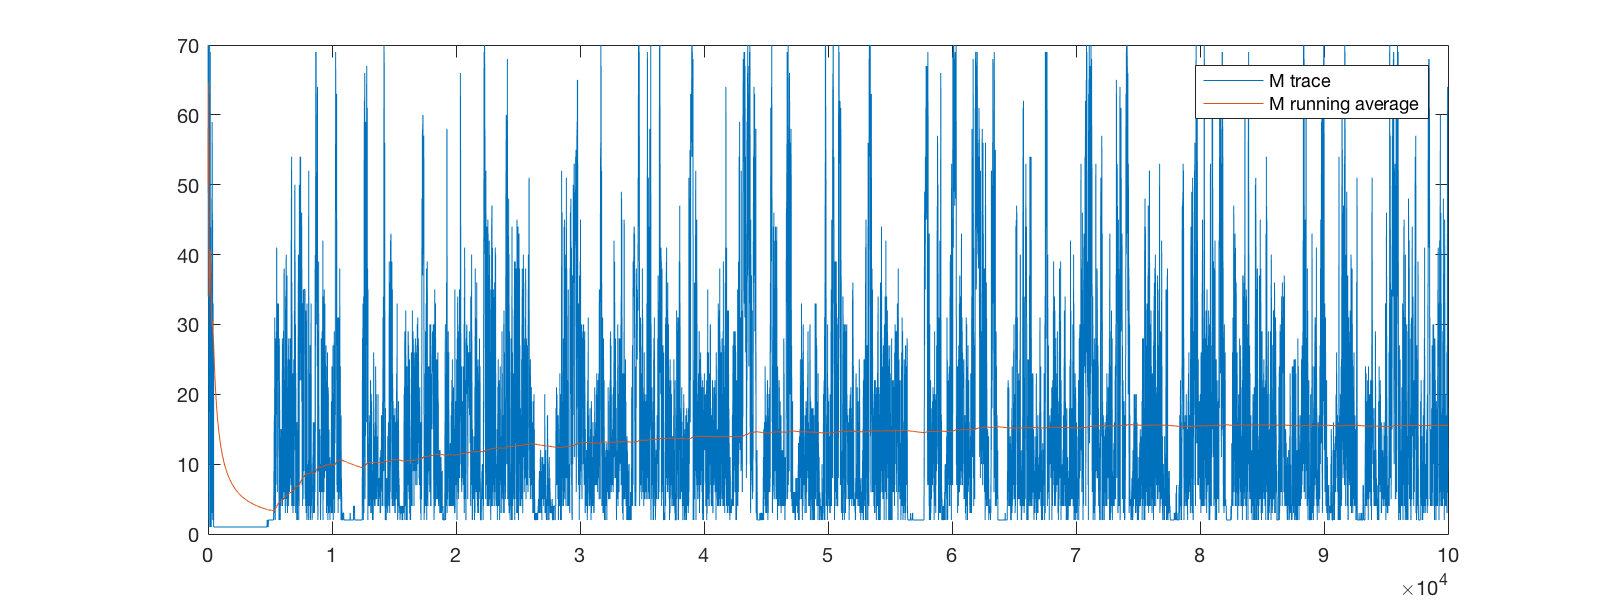
\includegraphics[width=\linewidth]{moons/hier1/M_trace.png}
\end{minipage} \hfill
\begin{minipage}{0.48\textwidth}
    \centering
    \caption{\label{fig:moons_hier1_M_accept} Hierarchical, seed $\text{rng}(3)$. $M$ accept.}
    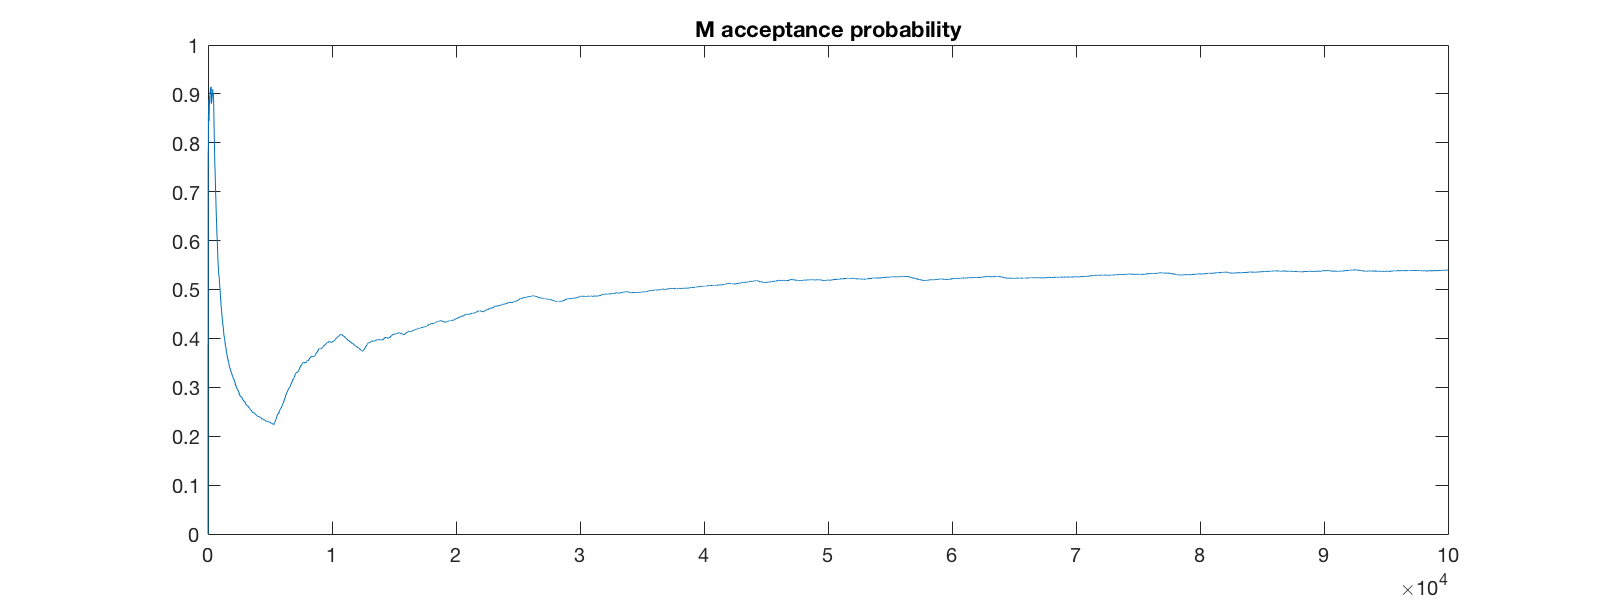
\includegraphics[width=\linewidth]{moons/hier1/M_accept.png}
\end{minipage}
\end{figure}


% rng(4)

\begin{figure}[!htb]
\begin{minipage}{0.48\textwidth}
    \centering
    \caption{\label{fig:moons_nonhier2_scatter} Nonhierarchical, seed $\text{rng}(4)$. Final classification projected into first two dimensions.}
    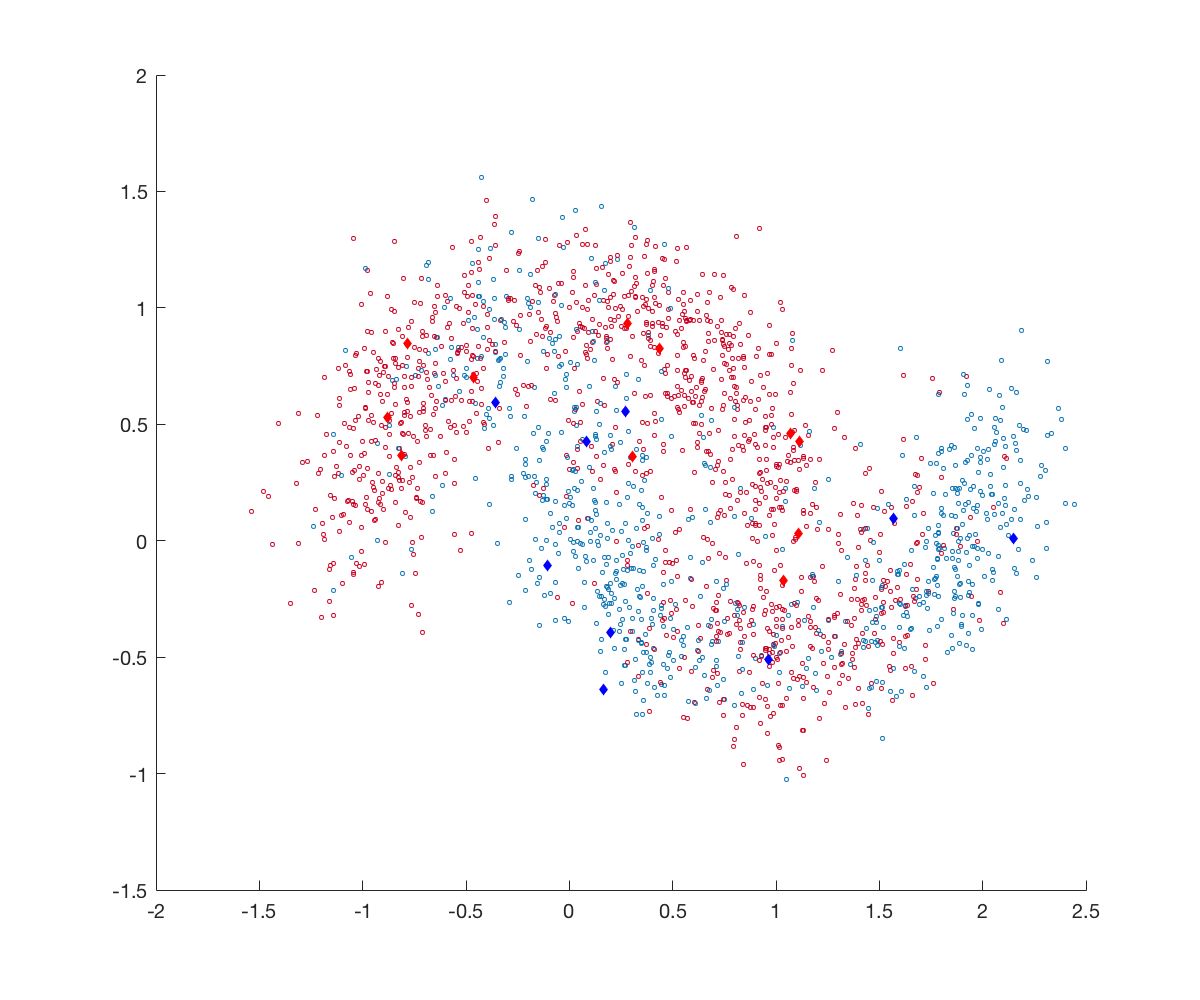
\includegraphics[width=\linewidth]{moons/nonhier2/scatter.png}
\end{minipage} \hfill
\begin{minipage}{0.48\textwidth}
    \centering
    \caption{\label{fig:moons_nonhier2_u_accept} Nonhierarchical, seed $\text{rng}(4)$. $u$ acceptance probability.}
    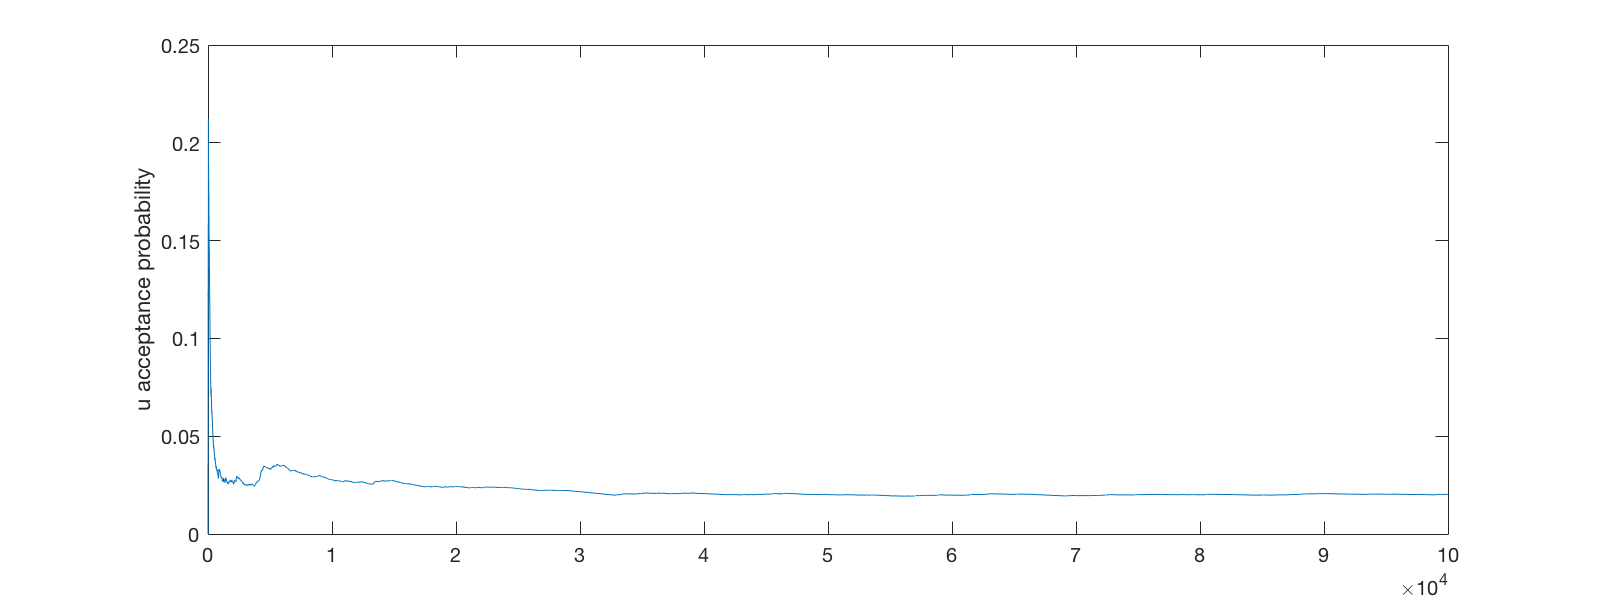
\includegraphics[width=\linewidth]{moons/nonhier2/u_accept.png}
\end{minipage}
\end{figure}

\begin{figure}[!htb]
\begin{minipage}{0.48\textwidth}
    \centering
    \caption{\label{fig:moons_hier2_scatter} Hierarchical, seed $\text{rng}(4)$. Final classification projected into first two dimensions.}
    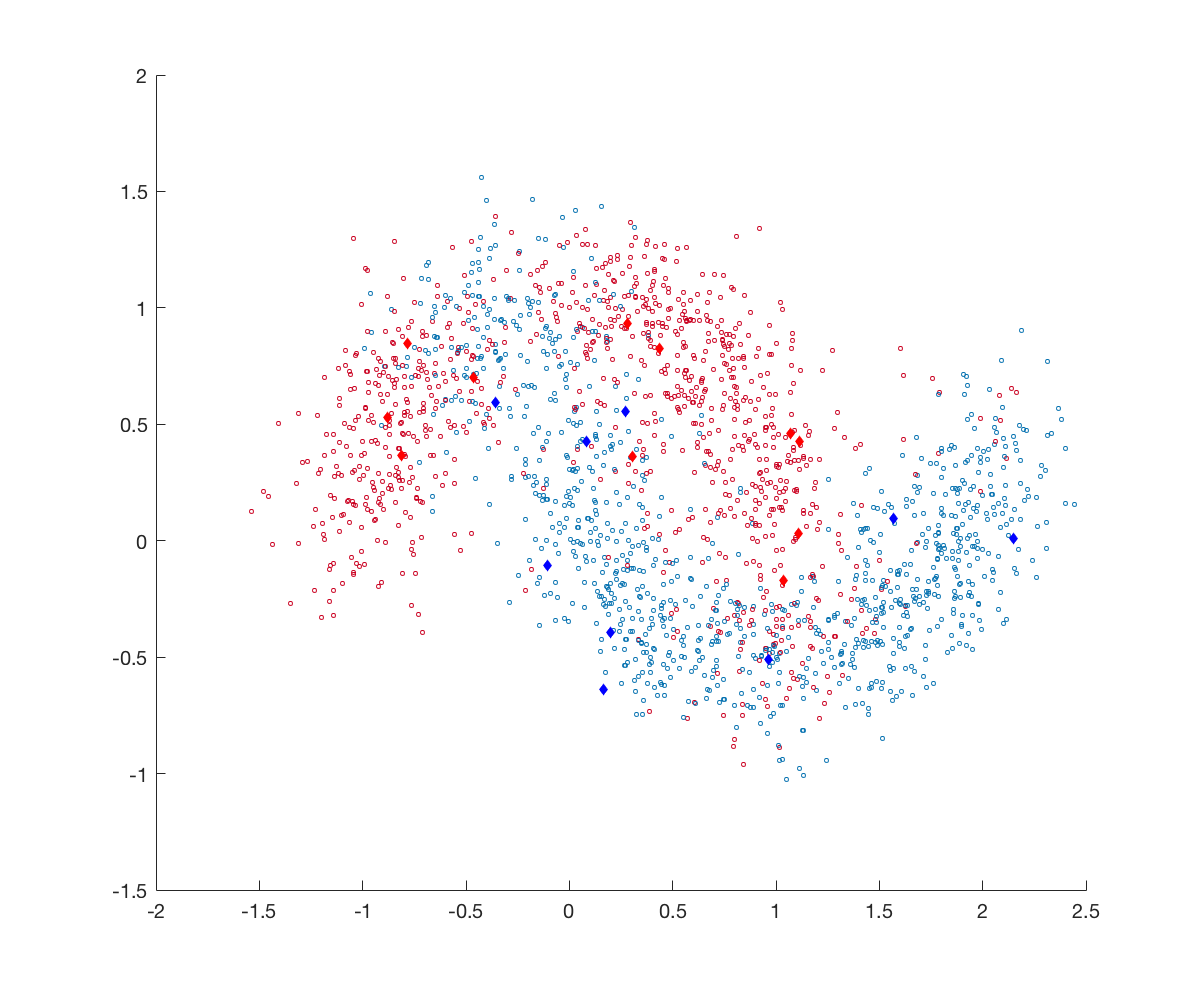
\includegraphics[width=\linewidth]{moons/hier2/scatter.png}
\end{minipage} \hfill
\begin{minipage}{0.48\textwidth}
    \centering
    \caption{\label{fig:moons_hier2_u_accept} Hierarchical, seed $\text{rng}(4)$. $\xi$ acceptance probability.}
    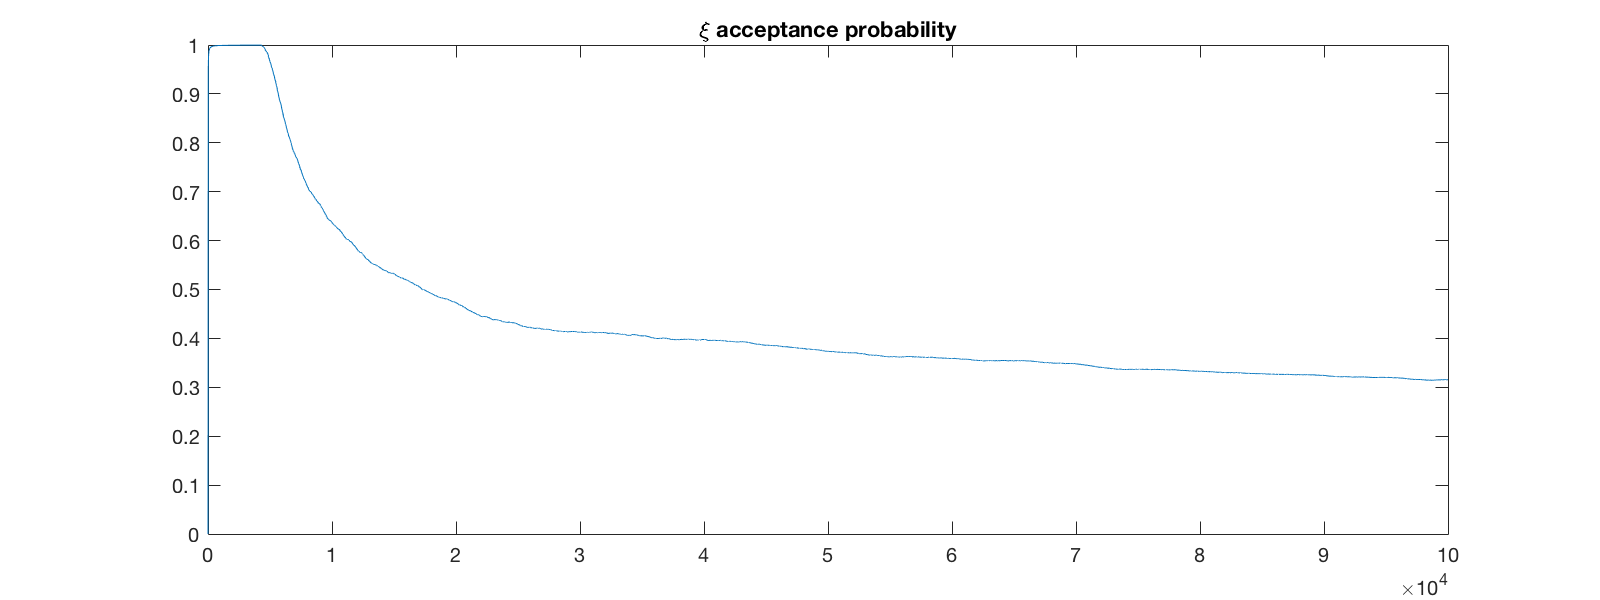
\includegraphics[width=\linewidth]{moons/hier2/xi_accept.png}
\end{minipage}
\end{figure}

\begin{figure}[!htb]
\begin{minipage}{0.48\textwidth}
    \centering
    \caption{\label{fig:moons_hier2_M_trace} Hierarchical, seed $\text{rng}(4)$. $M$ trace.}
    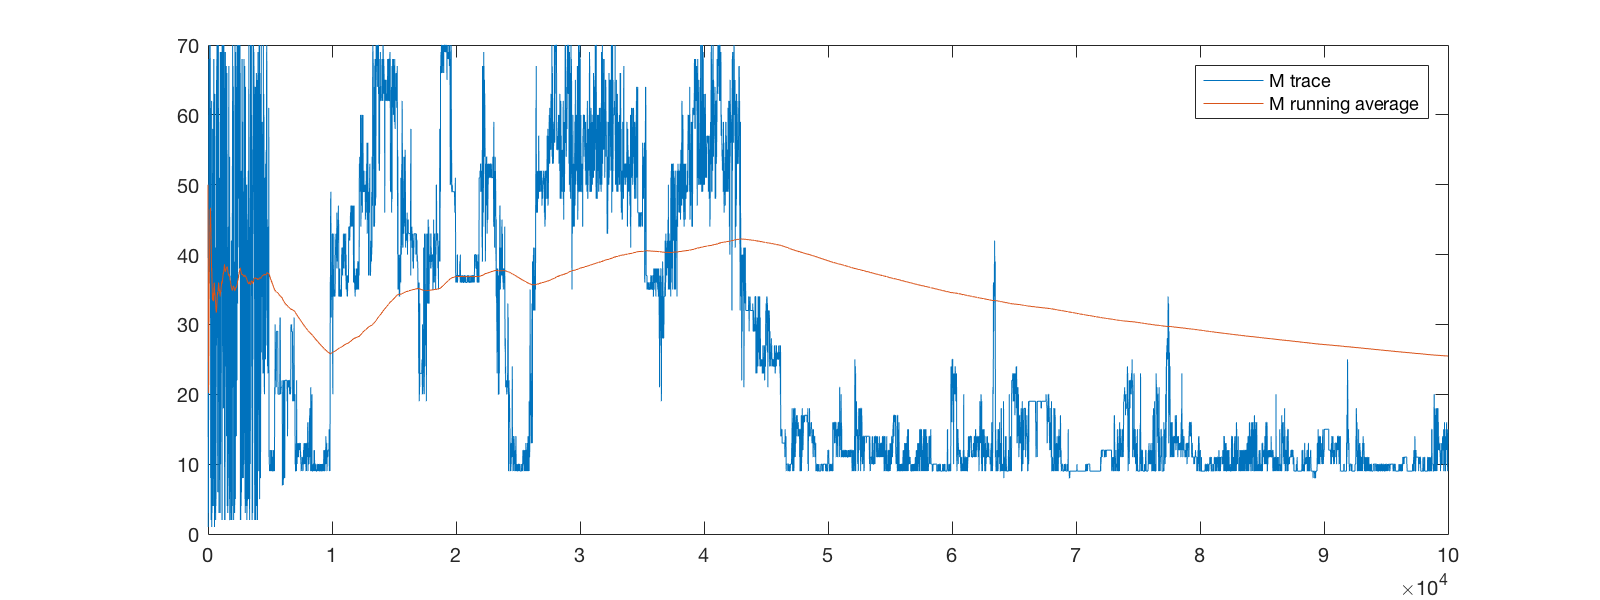
\includegraphics[width=\linewidth]{moons/hier2/M_trace.png}
\end{minipage} \hfill
\begin{minipage}{0.48\textwidth}
    \centering
    \caption{\label{fig:moons_hier2_M_accept} Hierarchical, seed $\text{rng}(4)$. $M$ accept.}
    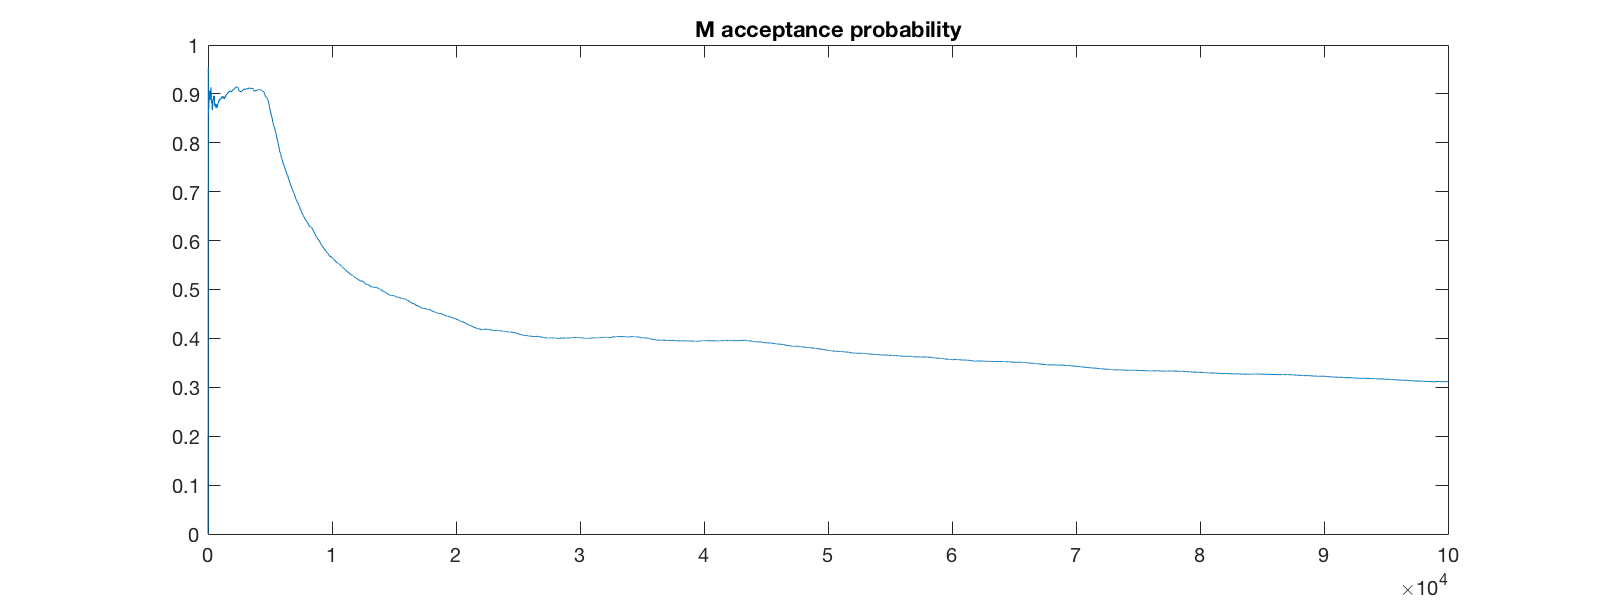
\includegraphics[width=\linewidth]{moons/hier2/M_accept.png}
\end{minipage}
\end{figure}

\bibliographystyle{siamplain}
\bibliography{references}
\end{document}